%Schriftgr�sse, Layout, Papierformat, Gleichungen Linksb�ndig
\documentclass[10pt,twoside,a4paper,fleqn]{article}
\usepackage[left=1cm,right=1cm,top=1cm,bottom=1cm,includeheadfoot]{geometry}
\usepackage[latin1]{inputenc}
\usepackage[ngerman]{babel,varioref}
%Packages - Von LinAlg Formelsammlung kopiert! �berpr�fen ob die alle notwendig sind
\usepackage{amsmath,amssymb,fancybox,graphicx,color,lastpage,wrapfig,fancyhdr,hyperref,verbatim}
\usepackage{listings}
%Package f�r Bilder im Fliesstext
\usepackage{multicol}

%Package f�r Tabelle im Querformat
\usepackage{rotating}

%Paragraphe ebenfalls nummerieren
\setcounter{secnumdepth}{4}



\raggedright
%Titel, Autor  
\newcommand{\titleinfo}{Zusammenfassung DT2}
\newcommand{\versioninfo}{$Revision: 218 $ - powered by \LaTeX}
\newcommand{\authorinfo}{G. K\"oppel, D. K\"oppel, S .K\"orner, C. Gwerder, L. Leuenberger}

%Seitenstyle

\pagestyle{fancy}
\fancyhf{}
%Kopfzeile links bzw. innen
\fancyhead[L]{\titleinfo{ }\tiny{(\versioninfo)}}
%Kopfzeile rechts bzw. aussen
\fancyhead[R]{Seite \thepage { }von \pageref{LastPage}}
%Fusszeile links bzw. innen
\fancyfoot[L]{\footnotesize{\authorinfo}}
%Fusszeile rechts bzw. ausen
\fancyfoot[R]{\footnotesize{\today}}


%Document Anfang
\begin{document}

\section{Realisierungs Methoden}
\subsection{ROM}
Mit einem ROM lassen sich sich rein kombinatorische Schaltungen in Form einer Look up Table realisieren.\\
\begin{itemize}
	\setlength{\itemsep}{1pt}
  \setlength{\parskip}{0pt}
  \setlength{\parsep}{0pt}
  
	\item Eingangsvariablen = Adresse\\
	\item Speicherwert = Ausgang (programmierbar)\\
\end{itemize}



\subsection{PLD}
Programmierbares Device aus AND und OR-Matrix, mindestens eine Matrix programmierbar.
\begin{itemize}
	\setlength{\itemsep}{1pt}
  \setlength{\parskip}{0pt}
  \setlength{\parsep}{0pt}
  
	\item PAL $\rightarrow$ OR-Matrix fest, AND-Matrix programmierbar, Fuses\\
	\item PLA $\rightarrow$ OR und AND Matrix frei programmierbar, Fuses\\
	\item GAL $\rightarrow$ Wie PLA plus programmierbare Ausgangsnetzwerke (Tristate), EEPROM\\
\end{itemize}
SPLD (Simple PLD): F"ur Funktionen die als DNF vorliegen geeignet, heute gr"osstenteils von CPLD und FPGA verdr"angt.\\

\subsection{CPLD (Complex PLD)}
\begin{itemize}
	\setlength{\itemsep}{1pt}
  \setlength{\parskip}{0pt}
  \setlength{\parsep}{0pt}
  
	\item Verbund PLD Makrozellen die mit Bussen verbunden sind, Speicherung der Konfiguration in Flash.\\
	\item	Durch regelm"assige Struktur sind Signallaufzeiten vorhersagbar.\\
	\item Wegen grosser Zahl an Logikbl"ocken sehr gut f"ur parallele Prozesse geeignet.\\
\end{itemize}

\subsection{FPGA}
2D-Array von Logikbl"ocken, die "uber Routing Kanal und Schaltmatrizen miteinander und mit I/O verbunden werden.\\
\begin{itemize}
	\setlength{\itemsep}{1pt}
  \setlength{\parskip}{0pt}
  \setlength{\parsep}{0pt}
  
	\item Logikblock (LogicCell) $\rightarrow$ Lookuptable mit D-FlipFlop, kann beliebige Funktionen ausf"uhren
	\item Schaltmatrizen $\rightarrow$ programmierbare Verbindungen
	\item Makrozellen $\rightarrow$ Feste Funktionen z.B. Memory, Clock Managment...
\end{itemize}
Die Konfiguration wird im RAM gespeichert (fl"uchtig). D.h. bei jedem Boot muss der Code von einem Festspeicher geladen werden.\\

%\subsection{Xilinx Spartan 3}
%\begin{itemize}
%	\setlength{\itemsep}{1pt}
%  \setlength{\parskip}{0pt}
%  \setlength{\parsep}{0pt}
%
%	\item Logic Cell (LC): Kleinste Einheit, enth"alt LUT mit 4 Eing"angen und eime D-FlipFlop. LUT kann als 16x1 bit SRAM oder Schieberegister 		konfiguriert werden. Zus"atzlich pro LC CarryLogic und MUX.
%	\item Slice: 1Slice = 2 Logic Cell
%	\item Configurable logic bloc (CLB): 1 CLB = 4 Slices = 8 Locic Cells. \\
%	Inerhalb dieser Einheit existieren spezifische Verbindungsstrukturen.
%\end{itemize}
%
%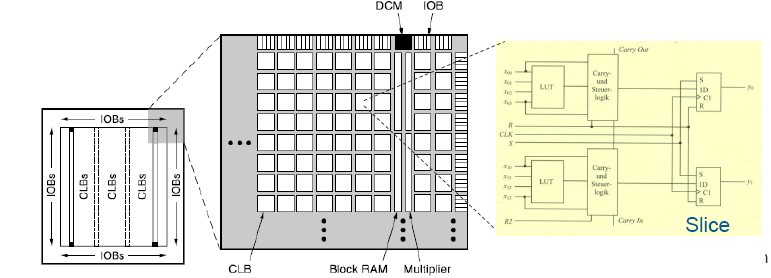
\includegraphics[width=0.8\textwidth]{pics/fpgastruct}


\subsection{Semicustom IC}
\begin{itemize}
	\setlength{\itemsep}{1pt}
  \setlength{\parskip}{0pt}
  \setlength{\parsep}{0pt}
  
	\item Mikrozellen aus p- und n-FETs werden durch Verdrahtung zu Gates 			
		$\rightarrow$Gate-Array/Sea of Gates\\
	\item Gates k"onnen durch Verdrahtungskan"ale verbunden werden.\\
	\item Standardfunktionen k"onnen mit IP (intelegent properity)-Cores implementiert werden.\\
	\item In Mixed-Signal Arrays sind zus"atzlich spezifische Analogbauteile enthalten\\
\end{itemize}	
	
\subsection{Fullcustom IC}
V"ollig kundenspezifische ICs, oft werden IP-Cores f"ur Standardfunktionen verwendet. Digitale und analoge Komponenten auf einem IC m"oglich. Voll auf Anwendung anpassbare Eigenschaften (Stromverbrauch, Gr"osse, Geschwindigkeit etc.).\\

\subsection{Vergeichstabelle}

\begin{center}
	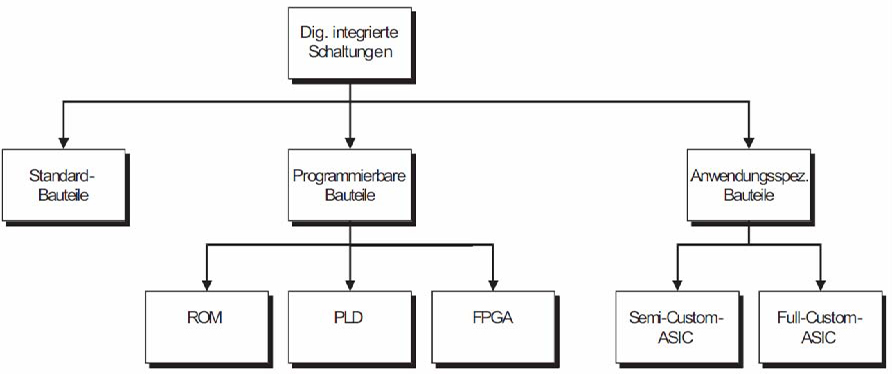
\includegraphics[width=0.40\textwidth]{pics/devicecomparetables}
	
	\begin{tabular}{|l|c|c|c|c|c|c|}
		\hline
		Kriterien & Standard Bauteile & ROM & PLD & FPGA & Semicustom & Fullcustom \\
		\hline
		Machbarkeit & ++ & - - & - - & + & + & +++ \\
		\hline
		Zeit Realisiertung & + & ++ & ++ & ++ & - & - - \\
		\hline
		Iterationszeit & - & ++ & ++ & ++ & - & - - \\
		\hline
		NRE & ++ & + & + & + & - & - - -\\
		\hline
		St"uckpreis & - - & + & + & - & + & +++ \\
		\hline
	\end{tabular}
\end{center}
	
\section{VHDL}
	Die vollst"andige Beschreibung des Designs (Grundstruktur) besteht aus:
	\begin{itemize}
	\setlength{\itemsep}{0pt}
  	\setlength{\parskip}{0pt}
  	\setlength{\parsep}{0pt}
		\item Bibliothekenbeschreibung [library]
		\item Schnittstellenbeschreibung [entity]
		\item Architekturbeschreibung [architecture]
	\end{itemize}

	\subsection{Key Concepts}
		\begin{tabular}{ll}
			Key Concept I: & Schaltungshierarchie und Verbindung von Sub-Bl"ocken 
				(hierarchy and connectivity).\\
			Key Concept II: & Nebenl"aufige (concurrent) Prozesse und Prozess-Interaktion.\\
			Key Concept III: & Modellierung des elektrischen Verhaltens von Signalen.\\
			Key Concept IV: & Event-Based time: Simulationsmodell, das auf Events und nicht 
				auf kontinuierlicher Zeit beruht.\\
			Key Concept V: & Parametrisierung von Modellen.
		\end{tabular}
	\subsection{Identifier}
		\begin{itemize}
			\setlength{\itemsep}{0pt}
  			\setlength{\parskip}{0pt}
  			\setlength{\parsep}{0pt}
				\item Start mit Buchstabe
				\item \_ nicht am Ende oder doppelt
				\item case insensitive
				\item Eigene Identifier $\rightarrow$ GROSSBUCHSTABEN
				\item Library Identifier $\rightarrow$ kleinbuchstaben
		\end{itemize}

	\subsection{Bibliotheken (library)}
		\begin{tabular}{ll}
			work & Default-Bibliothek des Benutzers \\
			std & standard (Vordefinierte Datentypen und Funktionen)\\
			& textio (Text -  Filehandling)\\
			work und std &m"ussen nicht deklariert werden (automatisch eingebunden)\\
			ieee & std\_logic\_1164: Datentypen f"ur mehrwertiges Logiksystem\\
			& numeric\_std: Mathe-Bibliothek f"ur std\_logic
		\end{tabular}
		\begin{multicols}{2}
			\lstinputlisting[language=VHDL,tabsize=2]{code/header.vhd}
		\end{multicols}
		 Mit \textbf{use} wird Bibliotheksinhalt im ganzen VHDL Modul sichtbar

	\subsection{Schnittstellenbeschreibung (entity)}
		Die einzelnen Bl"ocke einer VHDL-Beschreibung kommunizieren "uber ihre 
		Schnittstellen miteinander. Die Kommunikationskan"ale nach aussen sind die 
		sogenannten Ports. F"ur diese werden in der Schnittstellenbeschreibung Name, 		
		Signalflussrichtung und Datentyp festgelegt. Mit der Signalflussrichtung werden 
		Eing"ange (IN), Ausg"ange (OUT) und bidirektionale Ports (INOUT) unterschieden.
		\begin{multicols}{2}
			\lstinputlisting[language=vhdl,tabsize=2]{code/entity.vhd}
			\lstinputlisting[language=vhdl,tabsize=2]{code/entity_bsp.vhd}
		\end{multicols}

	\begin{multicols}{2}
	\subsubsection{Signalflussrichtungen (mode)}
		\begin{tabular}{ll}
			in: & Eingangssignal. Darf nur rechts stehen.\\
			out: & Ausgangssignal. Darf nur links stehen.\\
			buffer: & Ausgangssignal. Darf auch rechts stehen\\
			&  $\rightarrow$ \textbf{problematisch}\\
			inout: & Bidirektionales Signal, \\
			& in Verbindung mit Typ std\_logic.\\
		\end{tabular}
	\subsubsection{Signaltypen (type)}
		\begin{tabular}{ll}
			boolean & Werte: true, false\\
			bit & Werte: '0','1'\\
			bit\_vector: & eindimensionaler Array von bits\\
			integer & interne Darstellung mit 32bit\\
			& Range Einschr"ankung n"otig!\\
			std\_logic(\_vector) & wie bit(\_vector), f"ur mehrwertige Logik\\
			std\_ulogic(\_vetor) & wie std\_logic, nur f"ur einen Treiber\\
		\end{tabular}
	\end{multicols}
	
	\newpage
	
	\subsection{Architekturbeschreibung (architecture)}
		Die Architektur legt die Funktion eines Blocks fest. Dabei kann eine Entity mehrere 				Architecturen besitzen. Für das Erzeugen der FPGA-Programmierung sollten aber alle 
		nicht verwendeten Architekturen auskommentiert werden.
		\lstinputlisting[language=VHDL,tabsize=2]{code/architecture.vhd}

		\subsubsection{Signaldeklaration}
			 Hier werden die Signale, die Innerhalb der Architektur verwendet werden, 
			deklariert.
				\lstinputlisting[language=vhdl,tabsize=2]{code/signal.vhd}
			
		\subsubsection{Komponentendeklaration}
			Mit Hilfe des Schl"usselwortes \textbf{component} erfolgt die Deklaration von 
			Komponenten, "ahnlich wie einer \textbf{entity}.\\
%			Geschrieben wird das ganze beinahe gleich wie eine \textbf{entity} , nur wird 
%			das Wort \textbf{entity}  durch \textbf{component}  ersetzt, dass \textbf{is}
%			wird weggelassen und am Ende des Blocks wird mit \textbf{end component;} 	
%			abgeschlossen.
			\lstinputlisting[language=vhdl,tabsize=2]{code/component.vhd}
			
		\subsubsection{Anweisungsteil}
			Im Anweisungsteil wird das Verhalten beschrieben. Diese wird dabei 		
			durch verschiedene Modelierungsstile unterschieden.
			\begin{multicols}{2}
				\paragraph{Strukturmodell (Instanzierung)}
				Die Ein- und Ausgänge von Komponenten, die 
				in einer Bibliothek abgelegt sind werden durch lokale Signale miteinenander 
				verbunden $\rightarrow$ Es entsteht eine Netzliste. 
				\lstinputlisting[language=vhdl,tabsize=2]{code/instanzierung.vhd}
			
			
			\paragraph{Datenflussmodell}
				Es werden logische Grundfunktionen verwendet.
				Logikoperatoren f"ur bit, bit\_vector, boolean: \textbf{not, and, or, nand, nor,
 				xor, xnor	} Wenn auf bit\_vector angewendet, dann muss Bitbreite von 
				beiden Operanden gleich sein.

					\lstinputlisting[language=vhdl,tabsize=2]{code/datenfluss.vhd}
					
			\end{multicols}
			\paragraph{Verhaltensmodell} ($\rightarrow$ H"aufigster Modellierungsstil.) 
				Die Modellierung findet durch Sprachelemente "ahnlich wie in einer 	
				prozeduralen Programmiersprache statt.\\
				Dabei werden abgeschlossene Hardware-Bl"ocke durch Prozesse 
				abgebildet
				

	\subsection{Signalzuweisung}
		Alle Signalzuweisungen und alle Prozesse laufen parallel zueinander. 	
		Signalzuweisungen sind immer aktiv. Signale k"onnen auf verschiedene Arten 	
		zugewiesen werden:
		\begin{multicols}{2}
			\lstinputlisting[language=vhdl,tabsize=2]{code/signalzuweisung.vhd}
		\end{multicols}
		\subsubsection{Aggregat}
			Ein Aggregat ist ein Klammerausdruck, der mehrere Einzelelemente zu einem 
			Vektor zusammenfasst.
			\begin{multicols}{2}
			\lstinputlisting[language=vhdl,tabsize=2]{code/aggregat.vhd}
			\end{multicols}
		


	\subsection{Prozesse}
		\begin{multicols}{2}
			\begin{itemize}
			  \setlength{\itemsep}{1pt}
  			  \setlength{\parskip}{0pt}
  			  \setlength{\parsep}{0pt}
				\item Prozesse werden durch "Anderungen der Signale in der 	
					Sensitivit"atsliste aktiviert und ausgef"ahrt.
				\item Prozesse verhalten sich gegen aussen nebenl"aufig, innerhalb werden 
					Anweisungen sequentiell abgearbeitet
				\item \textbf{Selektive und bedingte Signalzuweisungen sind verboten.}
				\item Unbedingte Signalzuweisung sind erlaubt. 
				\item \textbf{Aktualisierung aller Signale geschieht immer erst am 
					Prozessende!}
				\item Zuweisen eines \textbf{Default-Wertes} an alle Ausgangssignale vor 	
					der ersten if-Anweisung zur Vermeidung von Latches 
				\item Hint: Damit Code "ubersichtlich und verst"andlich bleibt, sollte 	
					\textbf{nicht zu viel Funktionalit"at} in einen einzigen Prozess verpackt 
					werden.
				\item Alle Signale, die auf der rechten Seite einer Signalzuweisung stehen 	
					geh"oren in Sensitivit"atsliste 
				\item Ohne Sensitivit"atsliste nur in Simulation erlaubt
			\end{itemize}
			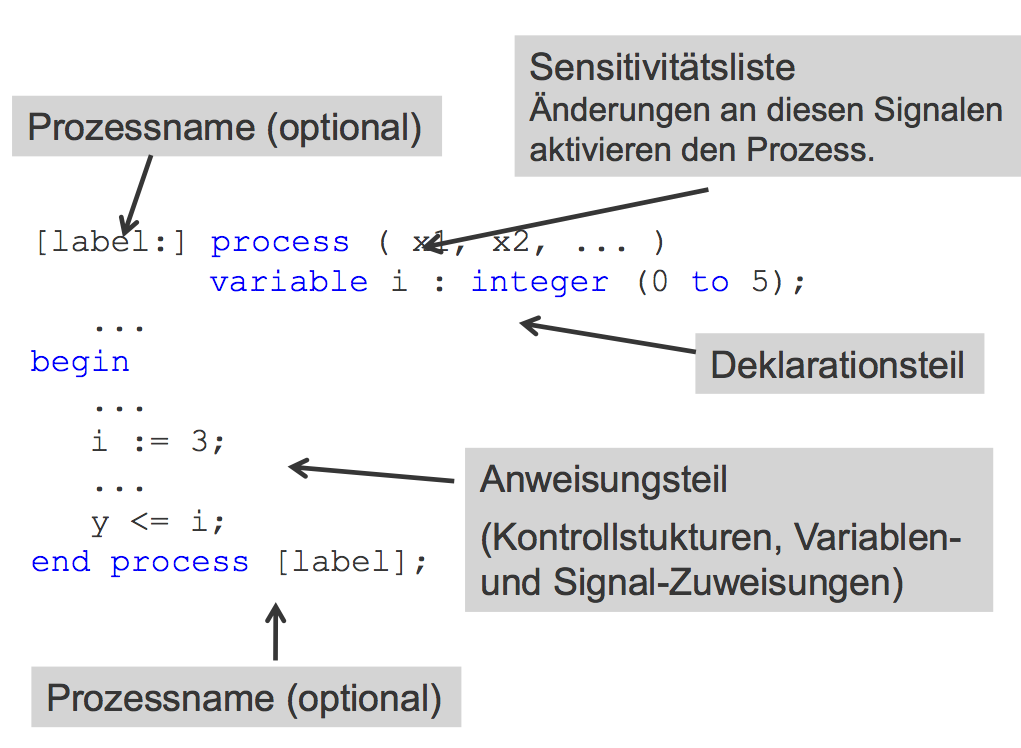
\includegraphics[width=0.535\textwidth]{pics/syntaxprozess}
		\end{multicols}
		
		\subsubsection{Variablen}
			\begin{multicols}{2}
				\begin{itemize}
					\item Variablen werden im Deklarationsteil des Prozesses deklariert 
						und nur in diesem Prozess sichtbar.
					\item Zugewiesener Wert kann sofort abgefragt werden
					\item Wertzuweisung durch Operator \textbf{:=} (nicht $<$=)
					\item Vor Verwendung ein aktueller Wert (evt. Default-Wert) zuweisen, 
						sonst entsteht Latch
				\end{itemize}
				\lstinputlisting[language=vhdl,tabsize=2]{code/variable.vhd}
			\end{multicols}

		\subsubsection{Signalzuweisung durch Prozesse}
			\begin{multicols}{2}
				\lstinputlisting[language=vhdl,tabsize=2]{code/kontrollstruktur.vhd}
			\end{multicols}

	\subsection{Sequentielle Systeme}
		\subsubsection{Flankenerfassung}
			\begin{multicols}{2}
				\lstinputlisting[language=vhdl,tabsize=2]{code/flanke.vhd}
			\end{multicols}
		\subsubsection{Zustandscodierung}
			\begin{multicols}{2}
				\begin{itemize}
					\item Die Deklaration der Zustandscodierung erfolgt im Deklarationsteil 						der Architektur
					\item Bei expliziten Zustandscodierung muss die Zustandcodierung der 
						IDE auf $"$User$"$ umgestellt werden.
				\end{itemize}
				\lstinputlisting[language=vhdl,tabsize=2]{code/zustandscode.vhd}
			\end{multicols}
		\subsubsection{FSM in 3-Prozess Struktur}
			Die Zustandsmaschine wird in 3 Prozesse aufgeteilt. Diese Prozesse werden ganz 
			einfach einzeln im Anwendungsteil der Architektur implementiert und arbeiten 
			jeweils nebenl"aufig.
			\begin{multicols}{2}
				\begin{center}
					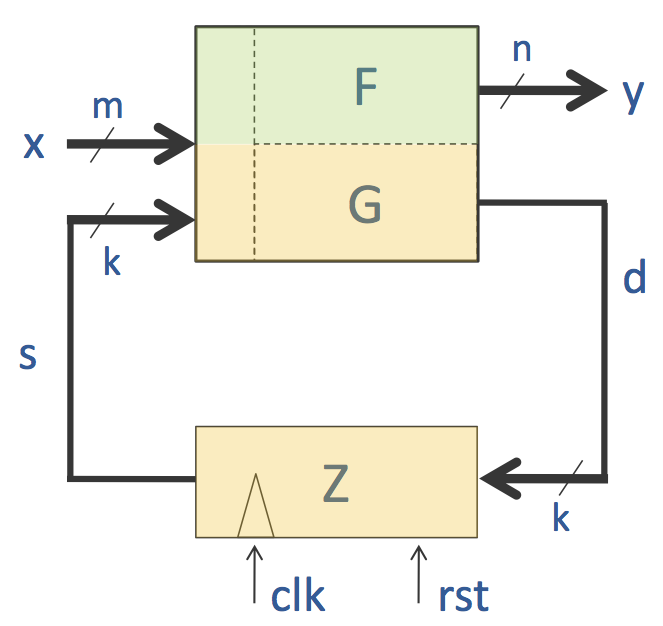
\includegraphics[width=0.15\textwidth]{pics/fsmprocesslogic}
				\end{center}
				\begin{itemize}
					\item Prozess F = Output\_Logic
					\item Prozess G = Next\_State\_Logic
					\item Prozess Z = State\_Register
				\end{itemize}
			\end{multicols}
			\paragraph{Output\_Logic}  $\;$ \\
				\begin{multicols}{2}
					Dieser kombinatorische Teil ist abh"angig von der Struktur der FSM.
					\lstinputlisting[language=vhdl,tabsize=2]{code/outputlogic.vhd}
				\end{multicols}
			\begin{multicols}{2}
				\paragraph{Next\_State\_Logic}  $\;$ \\
					Dieser kombinatorische Teil ist nicht abh"angig von der Struktur der 
					FSM.
					\lstinputlisting[language=vhdl,tabsize=2]{code/nextstatelogic.vhd}
				\paragraph{State\_Register}  $\;$ \\
					Dieser kombinatorische Teil ist nicht abh"angig von der Struktur der 
					FSM und sieht bei allen (fast) FSM immer gleich aus.
					\lstinputlisting[language=vhdl,tabsize=2]{code/stateregister.vhd}
			\end{multicols}
	
	\begin{multicols}{2}
		\subsection{IEEE 1164 Logiksystem}
			Durch Einbinden der ieee.std\_logic\_1164 Library werden die std\_logic, sowie 
			std\_ulogic Datentypen verf"ugbar. Damit verbunden ist auch die 9-wertige Logik:
			\begin{center}
				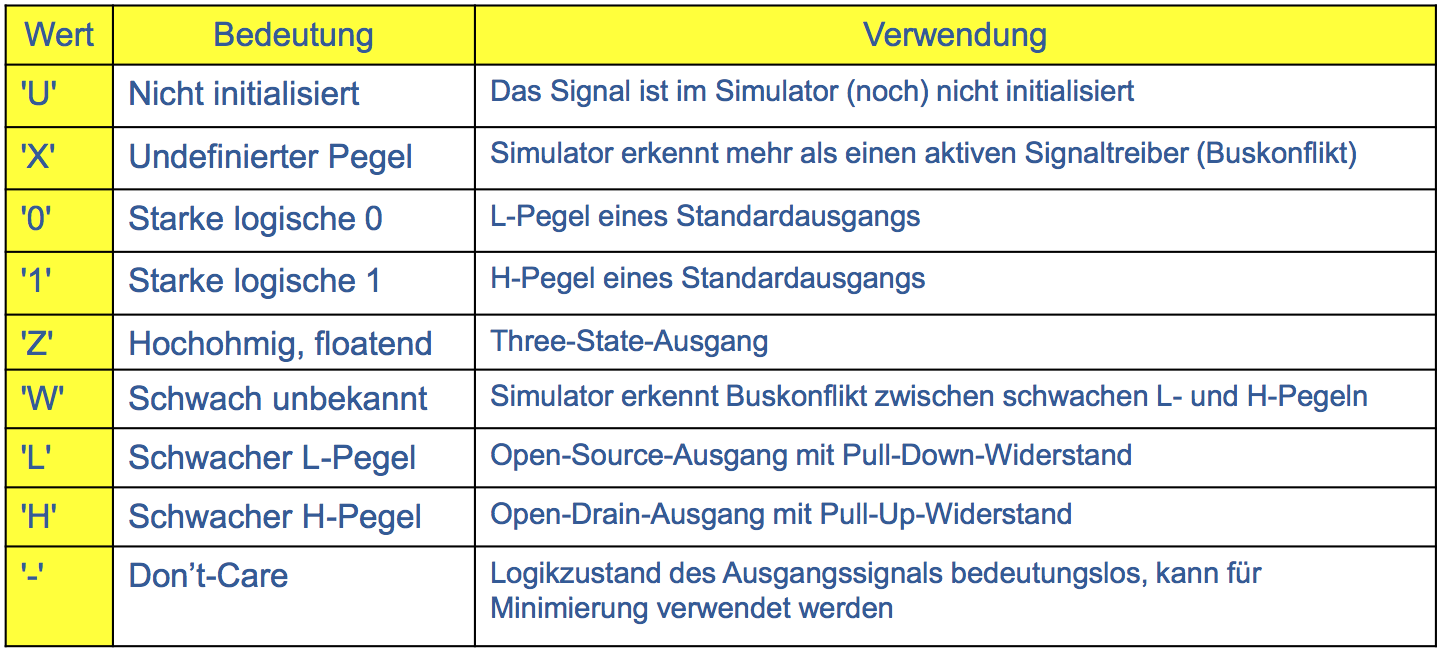
\includegraphics[width=0.4\textwidth]{pics/ieee1164logicsystem}
			\end{center}
		\subsubsection{Datentypenkonversion}
			Ebenfalls in der ieee.std\_logic\_1164 Library sind folgende Typenkonversionen 
			enthalten:
			\begin{center}
				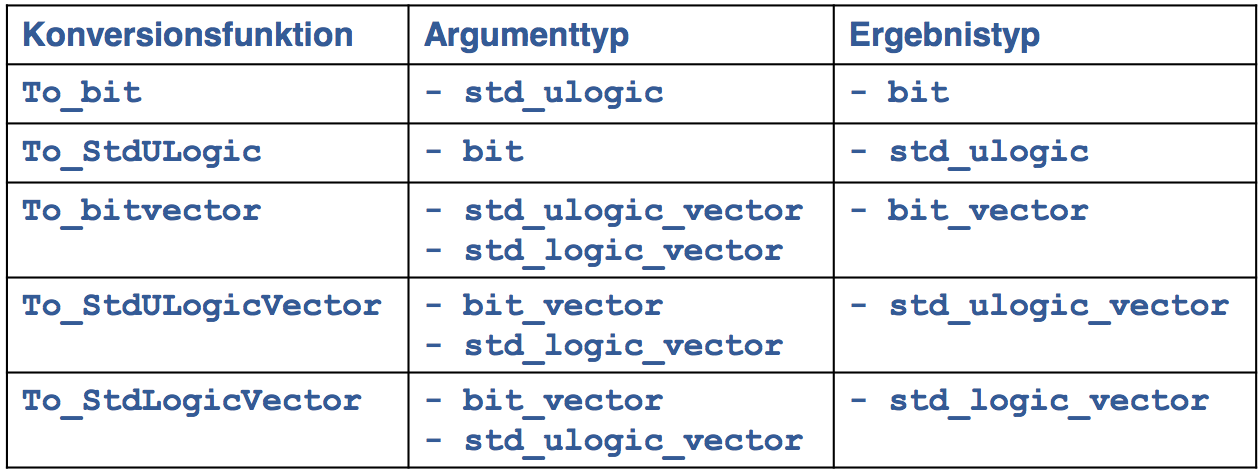
\includegraphics[width=0.3\textwidth]{pics/typeconversion}
			\end{center}
			\lstinputlisting[language=vhdl,tabsize=2]{code/typeconversion.vhd}
	\end{multicols}
	\subsection{Arithmetik}
		\begin{multicols}{2}
		Durch zus"atzliches Einbinden der ieee.numeric\_std neben ieee.std\_logic\_1164  	
		stehen signed und unsigned Datentypen auf Basis des std\_logic\_vector Datentyp, 
		sowie arithmetische Operatoren und Vergleichsfunktionen zur Verf"ugung.
		\begin{center}
			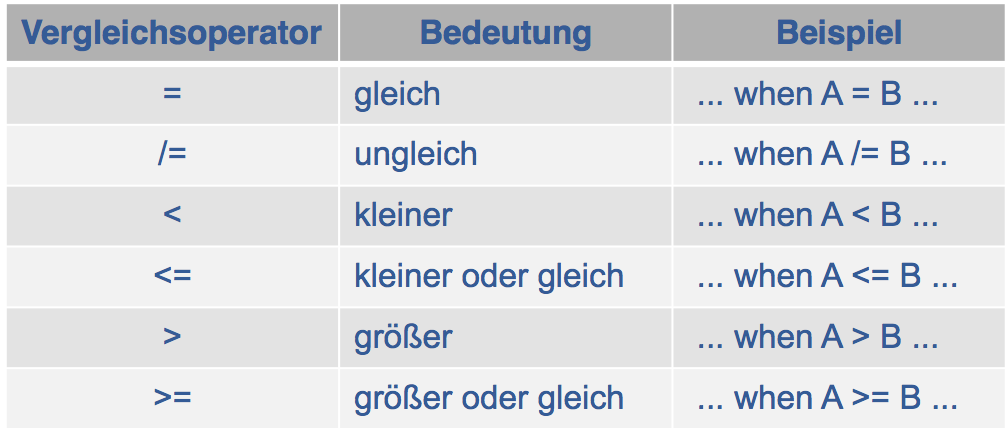
\includegraphics[width=0.3\textwidth]{pics/arithvergleich}
			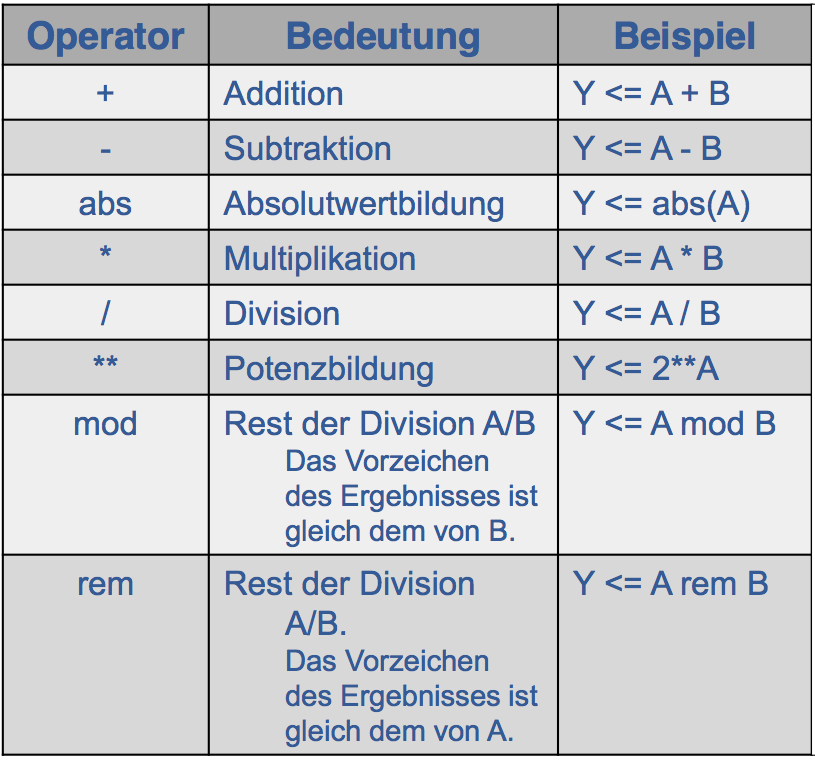
\includegraphics[width=0.25\textwidth]{pics/arithoperator}
		\end{center}
	\end{multicols}

	\subsection{Simulation}
		\subsubsection{Aufbau einer Test-Bench}
			\begin{multicols}{2}
				Normales VHDL Modul bestehend aus:
				\begin{itemize}
					\item library
					\item entity (i.d. Regel ohne Ports nach aussen)
					\item architecture
						\begin{itemize}
							\item Komponenten(DUT) deklerations
							\item ggf. Auswahl der DUT-Architektur
							\item (Timing-Informationen als Konstante (oder 
								Generic) deklarieren)
							\item Signale deklarieren(Bennenung: $<$DUT\_SIG$>$\_tb)
							\item Instanzierung der DUT
							\item Prozess f"ur Clock-Erzeugung
							\item Prozess f"ur die Anwendung von Stimuli 
								(Stimulusgenerator)
							\item Prozess f"ur das Erfassen der Systemantwort 
								(Response-Monitor)
						\end{itemize}
				\end{itemize}
			\end{multicols}

			\paragraph{DUT einbinden und konfigurieren (in Deklarationsteil)} $\;$ \\
				DUT wird als Komponente ganz normal deklariert.
				Sind mehrere Architekturen vorhanden, muss die zu stimulierende 	
				Architektur ausgew"ahlt werden:
				\lstinputlisting[language=vhdl,tabsize=2]{code/configarchitecture.vhd}
			\begin{multicols}{2}
				\paragraph{Timing-Konstante} $\;$ \\
					\lstinputlisting[language=vhdl,tabsize=2]{code/timeconstant.vhd}
				\paragraph{Clock-Prozess} $\;$ \\
					\lstinputlisting[language=vhdl,tabsize=2]{code/clockprozess.vhd}
				\paragraph{Stimulusgenerator} $\;$ \\
					\lstinputlisting[language=vhdl,tabsize=2]{code/stimulusgenerator.vhd}
			\end{multicols}	

			\paragraph{Response-Monitor (inkl. Assert)} $\;$ \\
				\lstinputlisting[language=vhdl,tabsize=2]{code/responsemonitor.vhd}
			
		\begin{multicols}{2}
			\subsubsection{For-Loop} % Evt. als paragraph, wenn Platzmangel
				For-Loops finden Verwendung in der Simulation, oftmals in Verbindung 
				mit wait-Statemants und daher ohne Sensititvit"atsliste.\\
				Sie k"onnen aber auch synthetisiert werden, daf"ur muss aber der range 
				endlich sein.
				\lstinputlisting[language=vhdl,tabsize=2]{code/forloop.vhd}
			\subsubsection{Verz"ogerungszeiten}  % Evt. als paragraph, wenn Platzmangel
				\begin{itemize}
					\item $\Delta$-Time $\rightarrow$ funktioneller Zusammenhang 
						zwischen Ursache/Wirkung (automatisch)
					\item inertial delay (Tr"agheit) $\rightarrow$Ausgang "andert erst, 
						wenn Eingang l"anger konstant bleibt als mit after definiert 
						(Nicht verwenden f"ur Verz"ogerungszeit)
						\lstinputlisting[language=vhdl,tabsize=2]
							{code/inertial.vhd}
					\item transport delay $\rightarrow$ Ausgang "andert nach 
						Eingans"anderung mit after definierter Zeit 
						\lstinputlisting[language=vhdl,tabsize=2]
							{code/transport.vhd}
				\end{itemize}
		\end{multicols}

	\subsection{Generic}
		$\rightarrow$ Re-Use! So kann VHDL mit Generic, Parameter an ein Modell 
		"ubergeben.\ Dabei wird der Parameter wie eine Konstante im Anweisungsteil 
		verwendet.\\
		Daf"ur muss in jeder Schnittstellenbeschreibung der Generic-Block eingbaut werden:
		\lstinputlisting[language=vhdl,tabsize=2]{code/generic.vhd}
		Und bei der Instanzierung wird mit generic map der Parameter-Wert gesetzt.
		\begin{multicols}{2}
			\subsubsection{Beispiel f"ur Implementation}
				Die Implemantation geschieht wie auch bei den anderen 
				Komponenten meistens in einer seperaten Datei, einfach enth"alt hier die 
				entity noch ein generic.
				\lstinputlisting[language=vhdl,tabsize=2]{code/generic_dekleration.vhd}
			\subsubsection{Beispiel f"ur Instanzierung}
				Auch hier wird wie gewohnt zu erst die Komponente deklariert und 
				anschliessend im Anwendungsteil instanziert.
				\lstinputlisting[language=vhdl,tabsize=2]{code/generic_instanzierung.vhd}
		\end{multicols}
		
%
%\subsection{VHDL Code Example}
%	\begin{center}
%		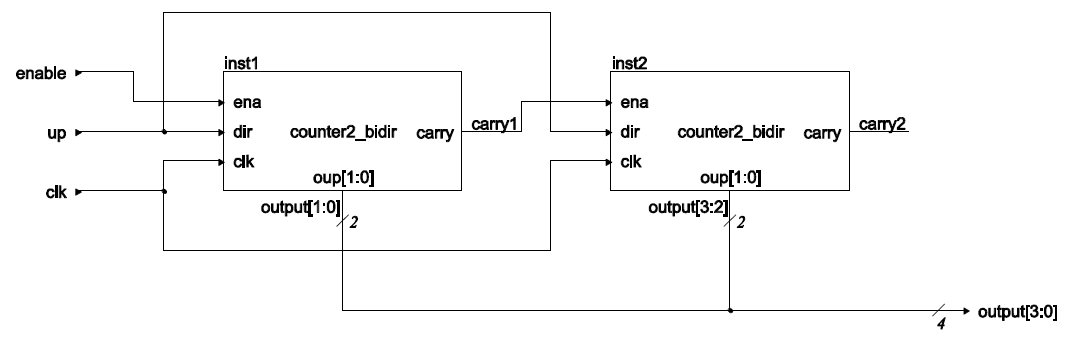
\includegraphics[width=0.5\textwidth]{pics/vhdlcodeexampleschematic.png}
%	\end{center}
%	\begin{multicols}{2}
%		\lstinputlisting[language=vhdl,tabsize=2]{code/vhdlcodeexample.vhd}
%	\end{multicols}
%
%
%
%
%\begin{center}
%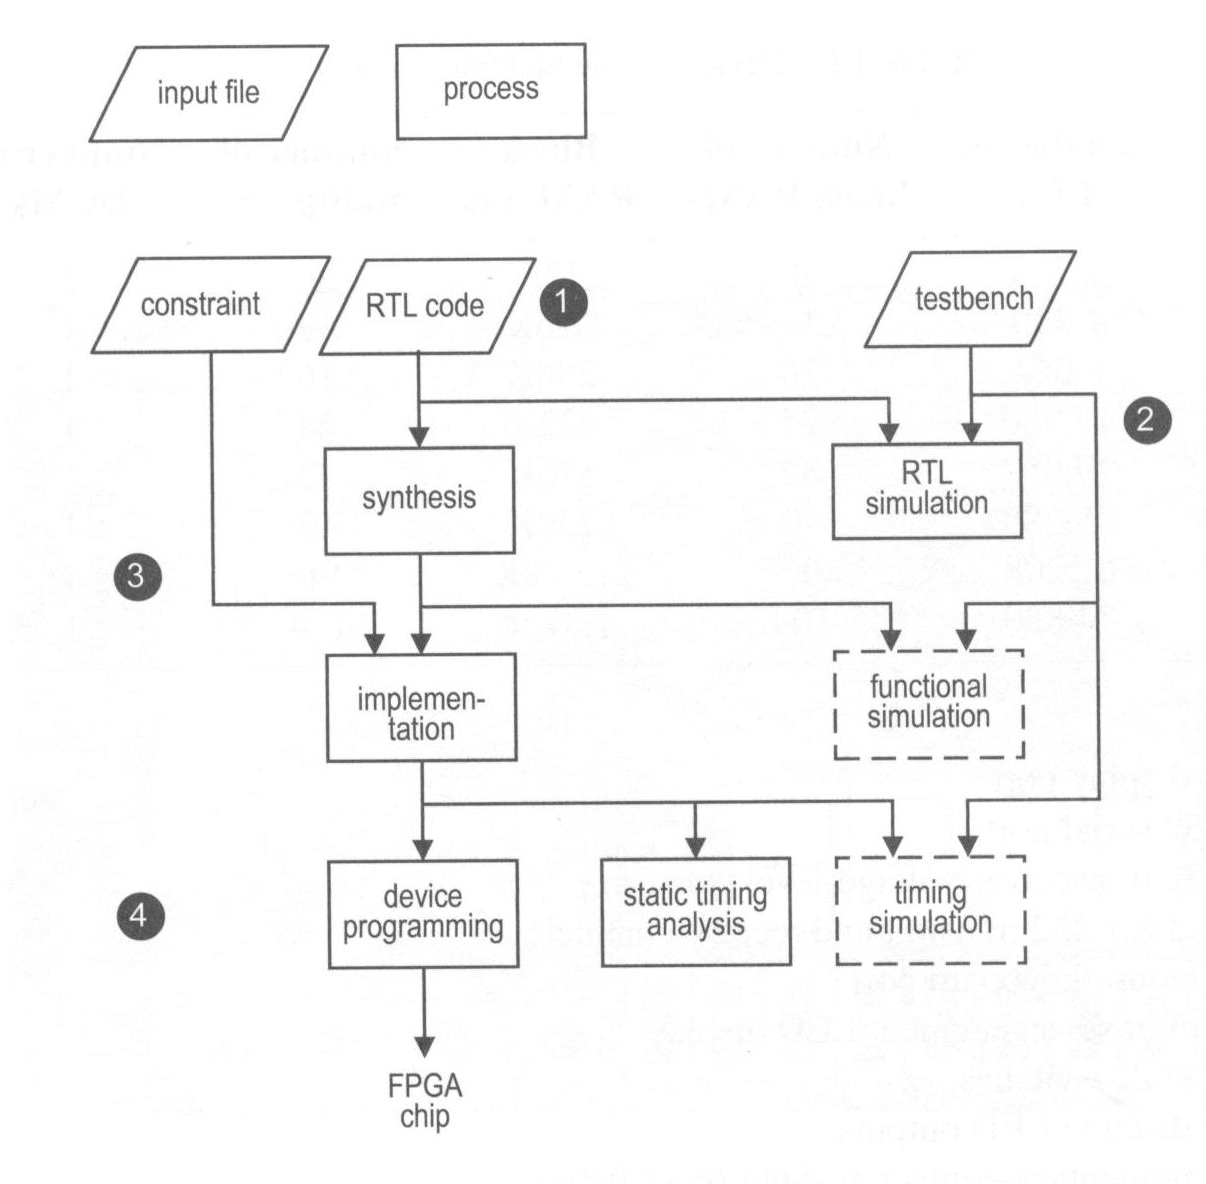
\includegraphics[width=0.5\textwidth]{pics/designprocess}
%\end{center}		

\end{document}
